%%%%%%%%%%%%%%%%%%%%%%%%%%%%%%%%%%%%%%%%%
% Simple Sectioned Essay Template
% LaTeX Template
%
% This template has been downloaded from:
% http://www.latextemplates.com
%
% Note:
% The \lipsum[#] commands throughout this template generate dummy text
% to fill the template out. These commands should all be removed when 
% writing essay content.
%
%%%%%%%%%%%%%%%%%%%%%%%%%%%%%%%%%%%%%%%%%

%----------------------------------------------------------------------------------------
%	PACKAGES AND OTHER DOCUMENT CONFIGURATIONS
%----------------------------------------------------------------------------------------

\documentclass[12pt]{article} % Default font size is 12pt, it can be changed here

\usepackage{geometry} % Required to change the page size to A4
\geometry{a4paper, left={40mm}, right={40mm}, top={25mm}, bottom={25mm},includehead,includefoot} % Set the page size to be A4 as opposed to the default US Letter

\usepackage{graphicx} % Required for including pictures

\usepackage{float} % Allows putting an [H] in \begin{figure} to specify the exact location of the figure
\usepackage{wrapfig} % Allows in-line images such as the example fish picture

\usepackage{lipsum} % Used for inserting dummy 'Lorem ipsum' text into the template

\usepackage{amsfonts}
\usepackage{amsmath}

\usepackage{listings}
\usepackage{listings-golang}
\lstset{
	basicstyle=\footnotesize\ttfamily,%
	breaklines=true,%
	captionpos=b,                    % sets the caption-position to bottom
	tabsize=2,	                   % sets default tabsize to 2 spaces
	%keywordstyle=\color{red},
}

\usepackage{hyphenat}
\usepackage{hyperref}

\usepackage{xcolor}
\hypersetup{
    colorlinks,
    linkcolor={red!50!black},
    citecolor={blue!50!black},
    urlcolor={blue!80!black}
}

\usepackage[sorting=none]{biblatex}
\addbibresource{bibliografia.bib}

\usepackage{pgfplots}

% ---------------------------------------------------------------------------------------
%	TIPOGRAFÍA
% ---------------------------------------------------------------------------------------

\usepackage[no-math]{fontspec}
\setmainfont[
	Path=./../fuentes/, 
	UprightFont=* Regular, 
	ItalicFont=* Italic,
	BoldFont=* Bold,
  	BoldItalicFont=* Bold Italic,
]{Equity Text A}
\setsansfont[
	Path=./../fuentes/, 
	UprightFont=* Regular, 
	ItalicFont=* Italic,
	BoldFont=* Bold,
  	BoldItalicFont=* Bold Italic,
]{Concourse T3}
\setmonofont[
	Path=./../fuentes/, 
	UprightFont=* Regular,% 
	%ItalicFont=* Italic,
	BoldFont=* Bold,
  	%BoldItalicFont=* Bold Italic,
  	SizeFeatures={Size=10.5},
]{FiraCode}

\usepackage[math-style=TeX]{unicode-math}
%\setmathfont{XITS Math}
\setmathfont[Path=./../fuentes/]{XITS Math}
\setmathfont[
	Path=./../fuentes/,
	range=up/{latin,Latin, num},
]{Equity Text A Regular}
\setmathfont[
	Path=./../fuentes/,
	range=it/{latin,Latin},
]{Equity Text A Italic}
\setoperatorfont\symup

\defaultfontfeatures{Ligatures=TeX,Numbers=Lining}


% ---------------------------------------------------------------------------------------
% 	CONFIGURACIÓN DEL ÍNDICE
% ---------------------------------------------------------------------------------------

\usepackage{titletoc}

\contentsmargin[0cm]{0cm}
\titlecontents{chapter}[0em]{\vskip12pt\bfseries\sffamily}
{\thecontentslabel\enspace}
{\hspace{1.05em}}
{ \hfill\contentspage}[\vskip 6pt]

\titlecontents{section}[1em]{\sffamily}
{\thecontentslabel\enspace}
{}
{\titlerule*[1pc]{.}\quad\contentspage}[\vskip 4pt]

\titlecontents{subsection}[2em]{\sffamily}
{\thecontentslabel\enspace}
{}
{\titlerule*[1pc]{.}\quad\contentspage}[\vskip 3pt]

\titlecontents{subsubsection}[4em]{\sffamily}
{\thecontentslabel\enspace}
{}
{\titlerule*[1pc]{.}\quad\contentspage}[\vskip 3pt]

\usepackage{etoolbox}
\pretocmd{\contentsname}{\sffamily}{}{}

% ---------------------------------------------------------------------------
% 	TÍTULOS DE PARTES Y SECCIONES
% ---------------------------------------------------------------------------

\usepackage{titlesec}

% Estilo de los títulos de las partes
\titleformat{\part}[hang]{\Huge\bfseries\sffamily}{\thepart\hspace{20pt}\textcolor{500}{|}\hspace{20pt}}{0pt}{\Huge\bfseries}
\titlespacing*{\part}{0cm}{-2em}{2em}[0pt]

% Reiniciamos el contador de secciones entre partes (opcional)
\makeatletter
\@addtoreset{section}{part}
\makeatother

% Estilo de los títulos de las secciones, subsecciones y subsubsecciones
\titleformat{\section}
  {\LARGE\bfseries\sffamily}{\thesection}{0.5em}{}

\titleformat{\subsection}
  {\Large\sffamily}{\thesubsection}{0.25em}{}

\titleformat{\subsubsection}
  {\large\sffamily}{\thesubsubsection}{0.25em}{}

 \usepackage[spanish]{babel}

\linespread{1.3} % Line spacing
\setlength{\parskip}{9pt}

\usepackage[bottom]{footmisc}

\renewcommand*\footnoterule{}

%----------------------------------------------------------------------------------------
%	CABECERAS Y PIES DE PÁGINA
%----------------------------------------------------------------------------------------

\usepackage{fancyhdr}
 
\pagestyle{fancy}
\fancyhf{}
\rfoot{\sffamily Página \thepage\ de \pageref{LastPage}}
\lfoot{\sffamily La web distribuida: el protocolo IPFS}

\renewcommand{\headrulewidth}{0pt}
\renewcommand{\footrulewidth}{0.5pt}

\usepackage{lastpage}

\setlength\parindent{0pt} % Uncomment to remove all indentation from paragraphs

\graphicspath{{Pictures/}} % Specifies the directory where pictures are stored

\usepackage[font=sf]{caption}

\begin{document}

%----------------------------------------------------------------------------------------
%	PÁGINA DEL TÍTULO
%----------------------------------------------------------------------------------------

\begin{titlepage}
\sffamily

\newcommand{\HRule}{\rule{\linewidth}{0.5mm}} % Defines a new command for the horizontal lines, change thickness here

\center % Center everything on the page

\textsc{\LARGE Universidad de Granada}\\[1.5cm] % Name of your university/college
\textsc{\Large Doble Grado en Ingeniería Informática y Matemáticas}\\[0.5cm] % Major heading such as course name
\textsc{\large Fundamentos de Redes}\\[0.5cm] % Minor heading such as course title

\HRule \\[1cm]
{ \huge \bfseries La web distribuida: el protocolo IPFS}\\[0.4cm] % Title of your document
\HRule \\[1.5cm]

\begin{minipage}{0.4\textwidth}
\begin{flushleft} \large
\emph{Autores:}\\
José María Martín Luque\\
Adolfo Soto Werner % Your name
\end{flushleft}
\end{minipage}
~
\begin{minipage}{0.4\textwidth}
\begin{flushright} \large
\emph{Profesor:} \\
Antonio Ruiz Moya\\ % Supervisor's Name
\hfill\\
\end{flushright}
\end{minipage}\\[4cm]

{\large \today}\\[3cm] % Date, change the \today to a set date if you want to be precise

%\includegraphics{Logo}\\[1cm] % Include a department/university logo - this will require the graphicx package

\vfill % Fill the rest of the page with whitespace

\end{titlepage}

%----------------------------------------------------------------------------------------
%	ÍNDICE
%----------------------------------------------------------------------------------------

\tableofcontents % Include a table of contents

\newpage % Begins the essay on a new page instead of on the same page as the table of contents 

%----------------------------------------------------------------------------------------
%	INTRODUCTION
%----------------------------------------------------------------------------------------

\section*{Introducción}

El Protocolo de transferencia de hipertexto (HTTP por sus siglas en inglés) es uno de los protocolos fundamentales de Internet. El desarrollo de HTTP comenzó en 1989 en el CERN por parte de Tim Berners-Lee. El desarrollo de un estándar fue un trabajo colaborativo entre el Grupo de Trabajo de Ingeniería de Internet (Internet Engineering Task Force, IETF) y el Consorcio WWW (World Wide Web Consortium, W3C), proceso que culminó con la publicación de una serie de \textit{Request for Comments} (RFCs)\footnote{Los RFCs son un tipo de documentos técnicos del IETF que datallan técnicamente diversos aspectos del funcionamiento de Internet y otros protocolos.}. La primera definición de \texttt{HTTP/1.1}, la versión de HTTP más utilizada, apareció en el RFC 2068 de 1997. 

Estamos hablando por tanto de un protocolo cuyo diseño comenzó hace más de 25 años. En aquel momento era inimaginable pensar que la tecnología que se estaba desarrollando fuese a ser usada por miles de millones de personas (3.885.567.619 a nivel mundial según las últimas estadísticas\cite{internet-world-stats} de junio de 2017) ni se esperaba que tuviese tal repercusión sobre nuestras vidas. HTTP ha simplificado y facilitado la transmisión de información a nivel mundial. Gracias a ello hemos avanzado hacia una sociedad conectada donde la información y la cultura fluye libremente.

Pero como es de esperar, un protocolo que no fue diseñado con la visión del mundo actual presenta una serie de problemas a resolver. La intención de este trabajo es mostrar las deficiencias de HTTP y explorar una alternativa a la web actual, la web distribuida y el protocolo IPFS.

\newpage


%----------------------------------------------------------------------------------------
%	CONTENIDO
%----------------------------------------------------------------------------------------

\section{Problemas de HTTP} % (fold)
\label{sec:problemas_de_http}

\subsection{Fragilidad} % (fold)
\label{sub:fragilidad}

\begin{figure}[h]
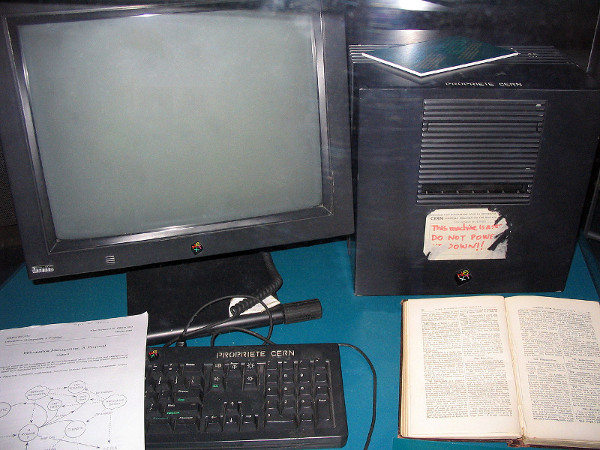
\includegraphics[width=\textwidth]{first-web-server}
\caption{Primer servidor de HTTP del mundo. Se trata del ordenador personal de Tim Berners-Lee durante su estancia en el CERN.}
\end{figure}

Para entender por qué decimos que HTTP es \textit{frágil} solo hay que observar la pegatina del primer servidor de HTTP: ``\textit{Esta máquina es un servidor. ¡¡No apagar!!}''. Está ahí para recordarnos que si se apagaba el servidor no se podía acceder al contenido. Otros sitios web en distintos servidores enlazaban a su contenido, de forma que si dejaba de estar en la red, todos esos enlaces no servían para nada. Por otro lado, si ese servidor se movía a otra ubicación, con otra dirección, todos esos enlaces habían muerto.

\begin{figure}[h]
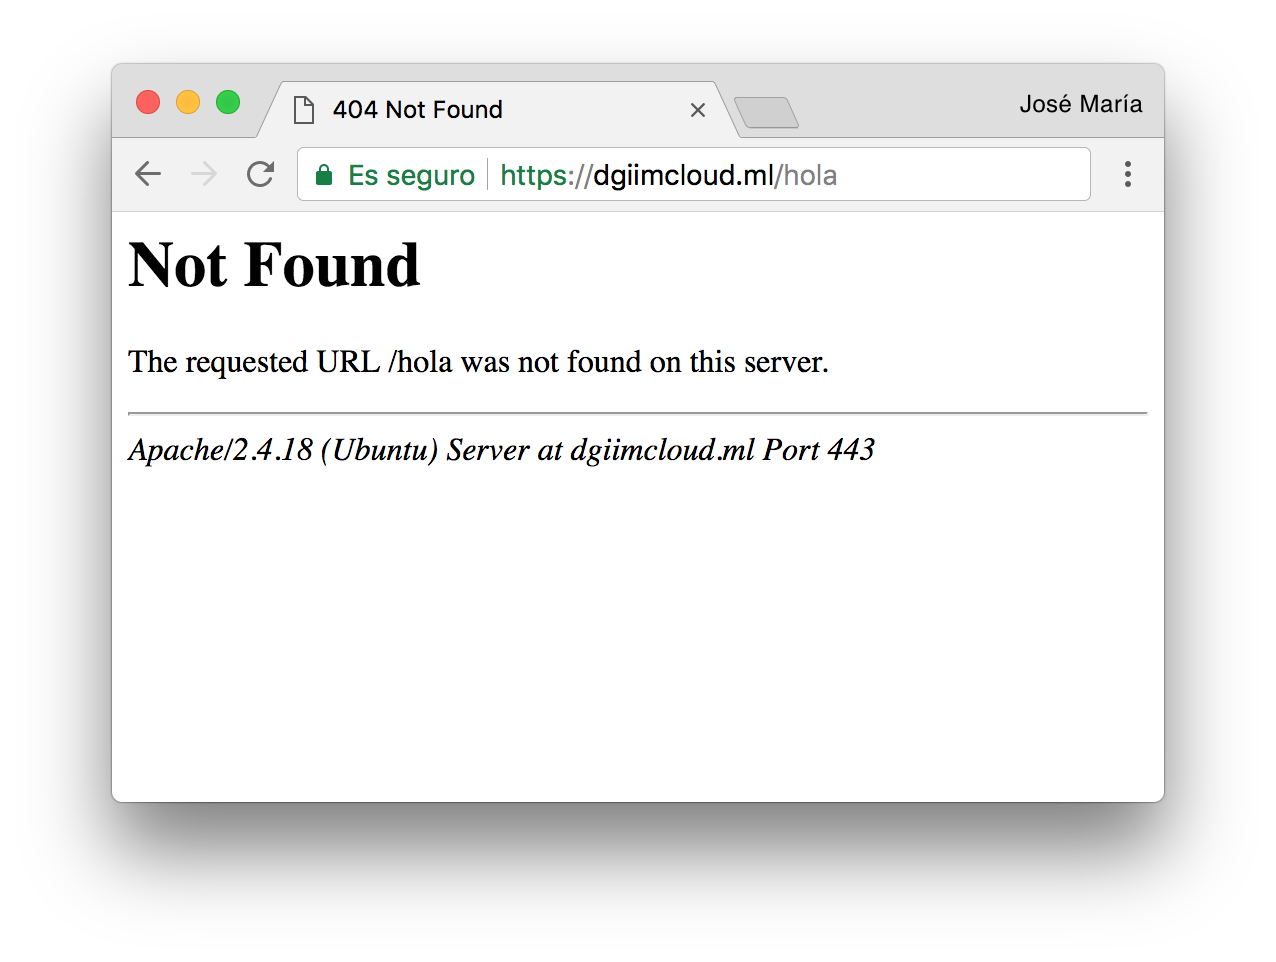
\includegraphics[width=\textwidth]{404}
\label{fig:404}
\caption{Error 404.}
\end{figure}

Hablamos en pasado pero efectivamente este sigue siendo un problema en la actualidad. No es raro entrar en algún enlace y encotrarnos con el error que podemos ver en la figura \ref{fig:404}. Incluso si no conoces la especificación del protocolo HTTP es probable que ya sepas que 404 es el código de error que nos indica que no hay nada que ver en una dirección.

La desaparición de enlaces (o \textit{link rot} en inglés) es mucho más habitual de lo que se pueda pensar. El creador de \href{pinboard.in}{Pinboard}, Maciej Cegłowski, estima que alrededor del 5\% de los enlaces que almacenan los usuarios en este servicio dejan de funcionar cada año\cite{pinboard-dead-links}. Añade además que uno de sus clientes ha visto cómo dejaban de funcionar el 90\% de los enlaces que llevaba almacenados desde 1997. En 2014, un estudio de Jonathan Zittrain, Kendra Albert y Lawrence Lessig de la Harvard Law School concluyó que aproximadamente el 50\% de los enlaces que aparecen en resoluciones del Tribunal Supremo de los Estados Unidos ya no redireccionan a la información original\cite{scotus-dead-links}. Por estos motivos existen servicios como \href{https://archive.org/}{The Internet Archive}, que se dedica a guardar copias de las páginas web para preservarlas de cara al futuro, o el propio Pinboard, que ofrece a sus usuarios la posibilidad de almacenar copias de los artículos que añadan al servicio.

% subsection fragilidad (end)

\subsection{Hipercentralización} % (fold)
\label{sub:hipercentralización}

En la \textit{Declaración de Independencia del Ciberespacio}\cite{cyberspace-independence} John Perry Barlow describía una utopía digital en la que los ciudadanos de la red se autogobiernan y las antiguas instituciones no tienen nada que hacer. ``De parte del futuro, os pido a vosotros del pasado que nos dejéis en paz. No sois bienvenidos entre nosotros. No tenéis la soberanía del lugar donde nos reunimos.'' 

Por desgracia, esta no es la realidad en el año 2017. En la actualidad la web está altamente centralizada. La práctica totalidad de los usuarios de Internet dependen de una serie de servicios concretos. Por poner algunos ejemlos, en 2015 Facebook anunció que más de mil millones de usuarios utilizaron el servicio en un mismo día\cite{billion-facebook}, mientras que una caída del servicio de Google en 2013 provocó una reducción del tráfico de internet del 40\%\cite{google-outage}.

El pasado 26 de octubre una inundación en la sala de servidores de la Universidad de Granada provocó que todos los servicios digitales dejasen de funcionar. Puede parecer algo leve pero gran parte de la actividad de la Universidad depdende de que funcione su infraestructura informática. Las secretarías dependen de la red, así como el servicio de comedores, las redes Wi-Fi (tienen que autenticar los usuarios en el servidor) y la Plataforma de Recursos de Apoyo a la Docencia (PRADO), entre otros.

La \textit{hipercentralización} de la red trae otras consecuencias negativas. Organizaciones como la NSA sólo tienen que intervenir el tráfico de unas pocas empresas para espiarnos, tal y como revelan las filtraciones de Edward Snowden\cite{snowden-leaks}. La censura es mucho más fácil de establecer ya que sólo hay que bloquear el acceso a una serie de sitios concretos. 

% subsection hipercentralización (end)

\subsection{Ineficiencia} % (fold)
\label{sub:ineficiencia}

Para comprobar la ineficiencia de transmitir información por HTTP vamos a poner un ejemplo. El vídeo más visto de YouTube según Wikipedia a 17 de octubre de 2017 es ``Luis Fonsi - Despacito ft. Daddy Yankee''\cite{most-viewed-yt}, con 4.055.733.709 visualizaciones a las 11:47.

Supongamos que el vídeo siempre se reprodujese en 720p, de tal forma que el archivo pesa exactamente 67,1MB. 4.055.733.709 visualizaciones de un archivo de 67,1MB son 272.139.731.874MB descargados. Suponiendo que a Google le costase 1 céntimo transmitir 1GB de información (incluyendo todos los gastos del servidor), ya se habría gastado más de 
272.139.731,874€ en transmitir un único vídeo.

Este precio de 1 céntimo por GB quizás sea posible para Google pero no lo es ni mucho menos para el ciudadano medio. La tabla de precios del CDN de Amazon, CloudFront es la siguiente\cite{cloudfront-prices}:

\begin{figure}[H]
	\centering
	\texttt{
\begin{tabular}{lrrrr}
  & Estados Unidos & Europa & Japón & India\\
  Primeros 10TB/mes & 0,085USD & 0,085USD & 0,140USD & 0,170USD\\
  Siguientes 40TB/mes & 0,080USD & 0,080USD & 0,135USD & 0,130USD\\
  Siguientes 100TB/mes & 0,060USD & 0,060USD & 0,120USD & 0,110USD\\
  Siguientes 350TB/mes & 0,040USD & 0,040USD & 0,100USD & 0,100USD\\
\end{tabular}}
	\caption{Tabla de precios de Amazon CloudFront en algunas regiones.}
\end{figure}
\vspace{-.5cm}
Podemos observar fácilmente que los precios son mucho mayores, ya que además se cobran las peticiones HTTP y HTTPS. La conclusión a la que queremos llegar es que a pesar de que HTTP ha abaratado muchísimo los costes de distribución de información, siguen siendo altos. Si el contenido a distribuir se encuentra en un servidor concreto, es necesario pagar los gastos generados tanto por distribuir el contenido como por el propio mantenimiento del servidor.


% subsection ineficiencia (end)

\subsection{Dependencia} % (fold)
\label{sub:dependencia}

Como ya hemos visto, Internet está actualmente \textit{hipercentralizado}. Esto implica que dependemos de una serie de infraestructuras clave para su correcto funcionamiento. En 2008 hubo problemas con una serie de cables submarinos de Internet, lo que conllevó que 14 países perdiesen la conexión, total o parcialmente\cite{2008-cable-disruption}.

% subsection dependencia (end)

% section problemas_de_http (end)

\section{La web distribuida} % (fold)
\label{sec:la_web_distribuida}

\subsection{Tecnologías de web distribuida} % (fold)
\label{sub:tecnologías_de_web_distribuida}

% subsection tecnologías_de_web_distribuida (end)

% section la_web_distribuida (end)

\section{El protocolo IPFS} % (fold)
\label{sec:el_protocolo_ipfs}

IPFS es un sistema de archivos distribuido que recoge algunas de las ideas más exitosas de otros sistemas \textit{peer to peer}. Los \textit{nodos} IPFS almacenan objetos en el almacenamiento local y se conectan entre sí para transferir dichos objetos, que representan archivos y otras estructuras de datos. El protocolo IPFS está dividido en una serie de sub-protocolos que se encargan de proporcionar distintas funciones.

\subsection{Identidades} % (fold)
\label{sub:identidades}

Se encarga de gestionar la generación y verificación de la identidad de los nodos. Los nodos se identifican por un \texttt{NodeId}, el \textit{hash} criptográfico de una clave pública, generado con S/Kademlia\footnote{Kademlia es un protocolo de la capa de aplicación diseñado para redes P2P descentralizadas. S/Kademlia es una mejora de este protocolo que pretende resolver algunos problemas que presentaba el original, entre ellos la asignación segura de \texttt{nodeId}\cite{S/Kamdelia}.}. Los nodos almacenan su clave pública y su clave privada, encriptada con una \textit{frase de contraseña}.

\begin{lstlisting}[caption={Definición de Nodo.}, language=Golang]
	// Hash criptográfico
	type NodeId Multihash
	type Multihash []byte
	
	// Claves
	type PublicKey []byte
	type PrivateKey []byte

	type Node struct {
		NodeId NodeID
		PubKey PublicKey
		PriKey PrivateKey
	}
\end{lstlisting}

\begin{lstlisting}[caption={Generación de identidad con S/Kamdelia.}, language=Golang]]
	difficulty = <parámetro integer>
	n = Node{}

	for cond := true; cond; cond = p < difficulty {
		n.PubKey, n.PrivKey = PKI.genKeyPair()
		n.NodeId = hash(n.PubKey)
		p = count_preceding_zero_bits(hash(n.NodeId))
	}
\end{lstlisting}

Cuando dos \textit{peers} se conectan, intercambian sus claves públicas y comprueban: \texttt{hash(other.PublicKey) == other.NodeId}. Si no es así, se cierra la conexión.

IPFS no utiliza una \textit{función hash} concreta, sino que utiliza valores \textit{autodescriptivos}. Así, los valores del \textit{hash digest} se guardan en el formato \textit{multihash}, que es de la forma:\\ 

\centerline{\texttt{<código función><longitud del digest><bytes del digest>}} 

Esto permite que el sistema escoja la mejor función para cada caso y evolucione conforme cambien las opciones.

% subsection identidades (end)

\subsection{Red} % (fold)
\label{sub:red}

Los nodos IPFS se comunican frecuentemente con cientos de otros nodos en la red, potencialmente a través del vasto Internet. El subsistema de red de IPFS incluye las siguientes funciones:

\begin{itemize}
	\item Transporte: IPFS puede utilizar cualquier protocolo de transporte, y es más adecuado para WebRTC DataChannels\footnote{Un canal de datos WebRTC te permite enviar texto o datos binarios a través de una conexión activa a un punto.\cite{WebRTC-data-channels}} (para conexión con navegadores) o µTP\footnote{Micro Transport Protocol (μTP) es un protocolo libre multiplataforma diseñado para ser usado en las conexiones P2P del protocolo BitTorrent. Está implementado sobre el protocolo UDP, como alternativa a TCP para la transferencia de datos.\cite{micro-transport-protocol}}.
	\item Fiabilidad: IPFS puede proporcionar fiabilidad si las redes subyacentes no lo proporcionan, usando µTP o SCTP.
	\item Conectividad: IPFS también utiliza las técnicas transversales ICE NAT\footnote{Interactive Connectivity Establishment (ICE) es una técnica usada en redes informáticas para encontrar formas de que dos ordenadores se comuniquen entre sí de la forma más directa posible en redes \textit{peer-to-peer}.\cite{interactive-connectivity-establishment}}.
	\item Integridad: opcionalmente se puede comprobar la integridad de los mensajes utilizando un \textit{checksum hash}.
	\item Autenticidad: opcionalmente se puede comprobar la autenticidad de los mensajes utilizando HMAC\footnote{Un código de autentificación de mensajes en clave-\textit{hash} (HMAC) es una construcción específica para calcular un código de autentificación de mensaje (MAC) que implica una función \textit{hash} criptográfica en combinación con una llave criptográfica secreta. Como cualquier MAC, puede ser utilizado para verificar simultáneamente la integridad de los datos y la autentificación de un mensaje.\cite{HMAC}} con la clave pública del remitente.
\end{itemize}

IPFS puede utilizar cualquier red: no depende ni asume acceso a IP. Esto permite utilizar IPFS en redes superpuestas\footnote{Una red superpuesta (\textit{overlay network}) es una red virtual de nodos enlazados lógicamente, que está construida sobre una o más redes subyacentes (\textit{underlying network}).\cite{red-superpuesta}}. IPFS almacena las direcciones como strings con formato byte \texttt{multiaddr} para que la red subyacente las utilice. \texttt{multiaddr} proporciona una forma de expresar direcciones y sus protocolos incluyendo soporte para encapsulación.

% subsection red (end)

\subsection{Enrutamiento} % (fold)
\label{sub:enrutamiento}

Los nodos IPFS requieren un sistema de enrutado que pueda encontrar tanto las direcciones de red de otros \textit{peers} como \textit{peers} que puedan distribuir objetos concretos. IPFS consigue esto utilizando una Tabla Hash Distribuida (DSHT por sus siglas en inglés) basada en S/Kamdelia y Coral\footnote{CoralCDN es una red de distribución de contenido (CDN por sus siglas en inglés) gratuita y abierta basada en tecnologías \textit{peer-to-peer} compuesta por una red mundial de \textit{proxies} web y \textit{nameservers}.}. Los datos pequeños (menores o iguales a \texttt{1KB}) se almacenan directamente en la DSHT. Para datos mayores, la DSHT almacena referencias, que son los \texttt{NodeIds} de los \textit{peers} que pueden distribuir el bloque en cuestión.

\begin{lstlisting}[caption={Interfaz de la DSHT.}, language=Golang]
	type IPFSRouting interface {
		// Obtiene la dirección de un nodo concreto
		FindPeer(node NodeId)

		// Almacena un pequeño dato en la DSHT
		SetValue(key []byte, value []byte)

		// Obtiene un pequeño dato de la DSHT
		GetValue(key []byte)

		// Anuncia que el nodo puede distribuir un dato grande
		ProvideValue(key Multihash)

		// Obtiene el número de peers distribuyendo un dato grande
		FindValuePeers(key Multihash, min int)
	}
\end{lstlisting}

Distintos casos de uso pueden requerir diferentes sistemas de enrutamiento, por lo que el sistema de enrutamiento de IPFS  puede cambiarse por uno que satisfaga las necesidades del usuario. Mientras que la interfaz descrita arriba se cumpla, el sistema continuará funcionando.

% subsection enrutamiento (end)

\subsection{Intercambio de bloques: el protocolo BitSwap} % (fold)
\label{sub:intercambio_de_bloques_el_protocolo_bitswap}

En IPFS la distribución ocurre intercambiando bloques con \textit{peers} utilizando un protocolo inspirado por BitTorrent: BitSwap. Como BitTorrent, los \textit{peers} de BitSwap buscan conseguir un conjunto de bloques (\texttt{want\_list}) y tienen otro conjunto de bloques que ofrecer (\texttt{have\_list}). Sin embargo, a diferencia de BitTorrent, BitSwap no se limita a una serie de bloques en un \textit{torrent}, sino que opera como un ``mercado'' donde los nodos pueden adquirir los bloques que necesitan, independientemente del archivo al que esos bloques pertenezcan. Esta idea requeriría que se implementase una moneda virtual, lo que haría necesario un control central sobre dicha moneda. IPFS implementa esto como la \textit{estrategia BitSwap}, que veremos a continuación.

En el caso base, los nodos BitSwap tienen que proporcionar un valor inmediato entre ellos en forma de bloques. Esto funciona bien cuando la distribución de bloques entre nodos es complementaria: cada uno de ellos tiene lo que necesita el otro. Sin embargo lo más probable es que esto no sea así. En algunos casos los nodos tienen que \textit{trabajar} para conseguir sus bloques. En el caso de que un nodo no tenga algo que quieran sus \textit{peers}, buscará las pizas que estos quieren, con una prioridad menor que los que el propio nodo quiere. Esto incentiva que los nodos almacenen en caché y distribuyan piezas más raras, incluso si no están interesadas en ellas directamente.

\subsubsection{Crédito BitSwap} % (fold)
\label{ssub:crédito_bitswap}

El protocolo también debe incentivar que los nodos \textit{siembren}\footnote{Del inglés \textit{to seed}, en este caso significa distribuir información.} cuando no necesitan nada en particular, puesto que pueden tener bloques que otros nodos quieran. Los nodos BitSwap envían bloques a sus \textit{peers} de forma optimista, esperando que la \textit{deuda} se les pague en un futuro. Sin embargo, también hay que protegerse de los \textit{leeches}, nodos que nunca comparten. Un sistema de créditos resuelve el problema:
\begin{enumerate}
	\item Los \textit{peers} realizan un seguimiento de su saldo (en bytes verificados) con otros nodos.
	\item Los \textit{peers} envían bloques a otros \textit{peers} deudores probabilísticamente, de acuerdo a una función que decrece conforme la deuda incrementa.
\end{enumerate}

Si un nodo decide no enviar bloques a un \textit{peer}, el nodo lo ignorará durante un tiempo \texttt{ignore\_cooldown} (10 segundos por defecto en BitSwap). Esto evita que se juegue con la probabilidad simplemente haciendo más peticiones.

% subsubsection crédito_bitswap (end)

\subsubsection{Estrategia BitSwap} % (fold)
\label{ssub:estrategia_bitswap}

Los \textit{peers} BitSwap pueden adoptar diferentes estrategias, que proporcionarán resultados muy variados en el intercambio de bloques. La elección de una función debería procurar:
\begin{enumerate}
	\item maximizar la actividad de intercambio del nodo.
	\item evitar que los \textit{leechers} se aprovechen del sistema y degraden el intercambio.
	\item sea efectiva y resistente a otras estrategias.
	\item ser clemente con \textit{peers} de confianza.
\end{enumerate}
Una elección de función que funciona en la práctica es una sigmoide, escalada por una \textit{ratio de deuda}:

Definimos la \textit{ratio de deuda}, \textit{r} entre un nodo y su \textit{peer} como:
\begin{equation*}
	r = \frac{\texttt{bytes\_enviados}}{\texttt{bytes\_recibidos} + 1}
\end{equation*}
Dado $r$, la probabilidad de enviar a un deudor es:
\begin{equation*}
	P(r) = 1 - \frac{1}{1 + exp(6-3r)}
\end{equation*}

\begin{figure}
	\centering
	\begin{tikzpicture}
		\begin{axis}[
			xlabel=$r$,
			ylabel={$P(r)$},
			xmin=0,xmax=4,
		]
		% use TeX as calculator:
		\addplot {1 - (1/(1 + pow(e, 6-3*x)))};
		\end{axis}
	\end{tikzpicture}
	\caption{Representación de la función de probabilidad $P(r)$.}
\end{figure}

Como se puede observar en la figura la función decrece fuertemente cuando la \textit{ratio de deuda} del nodo aumenta. Esta radio es una medida de confianza: clemente con las deudas de los nodos con los que se que han intercambiado grandes cantidades de datos e implacable con  aquellos desconocidos y que no son de confianza.

% subsubsection estrategia_bitswap (end)

\subsubsection{Libro mayor de BitSwap} % (fold)
\label{ssub:libro_mayor_de_bitswap}

Los nodos BitSwap mantienen una especie de ``libro mayor\footnote{Un \textit{libro mayor} es un libro de contabilidad en que se registran las partidas importantes o globales.}'' (\textit{ledger} en inglés) en el que se registran las transferencias con otros nodos. Cuando se inicia una conexión los nodos BitSwap intercambian su libro mayor. Si no concuerdan, el libro mayor se reinicia, perdiendo el crédito y la deuda. Es posible que hay nodos maliciosos que ``pierdan'' el libro mayor a propósito con el fin de borrar deudas. Es muy poco probable que un nodo acumule demasiada deuda como para querer perderla junto con la confianza, aunque otros nodos pueden considerarlo una mala conducta y negarse a intercambiar información.

\begin{lstlisting}[caption={Implementación del libro mayor.}, language=Golang]
	type Ledger struct {
		owner NodeId
		partner NodeId
		bytes_sent int
		bytes_recv int
		timestamp Timestamp
	}
\end{lstlisting}

% subsubsection libro_mayor_de_bitswap (end)

\subsubsection{Especificación de Bitswap} % (fold)
\label{ssub:especificación_de_bitswap}

Los nodos BitSwap siguien un protocolo simple.

\begin{lstlisting}[caption={Implementación del protocolo BitSwap}, language=Golang]
	// Estado adicional almacenado
	type BitSwap struct {
		// Libros mayores del nodo
		ledgers map[NodeId]Ledger

		// Conexiones abiertas actualmente
		active map[NodeId]Peer

		// Checksums de bloques que necesita el nodo
		need_list []Multihash

		// Checksums de bloques que tiene el nodo
		have_list []Multihash
	}

	type Peer struct {
		nodeid NodeId
		// Libro mayor entre el nodo y este peer
		ledger Ledger

		// Marca de tiempo del último mensaje recibido
		last_seen Timestamp

		// Checksums de los bloques que quiere el peer
		// Incluye bloques que quieren los peers del peer
		want_list []Multihash
	}

	// Interfaz del protocolo
	interface Peer {
		open(nodeid NodeId, ledger Ledger)
		send_want_list (want_list WantList)
		send_block (block Block) complete Bool
		close(final Bool)
	}
\end{lstlisting}

% subsubsection especificación_de_bitswap (end)

% subsection intercambio_de_bloques_el_protocolo_bitswap (end)

\subsection{Cómo soluciona IPFS los problemas de HTTP} % (fold)
\label{sub:cómo_soluciona_ipfs_los_problemas_de_http}

% subsection cómo_soluciona_ipfs_los_problemas_de_http (end)

% section el_protocolo_ipfs (end)

\section{La web distribuida en la actualidad} % (fold)
\label{sec:la_web_distribuida_en_la_actualidad}

\subsection{La Wikipedia descentralizada} % (fold)
\label{sub:la_wikipedia_descentralizada}

% subsection la_wikipedia_descentralizada (end)

\subsection{Neocities} % (fold)
\label{sub:neocities}

% subsection neocities (end)

\subsection{La web del referéndum ilegal sobre la independencia de Cataluña (2017)} % (fold)
\label{sub:la_web_del_referéndum_catalán_de_2017}

% subsection la_web_del_referéndum_catalán_de_2017 (end)

% section la_web_distribuida_en_la_actualidad (end)

%----------------------------------------------------------------------------------------
%	BIBLIOGRAFÍA
%----------------------------------------------------------------------------------------

\newpage
\printbibliography
%----------------------------------------------------------------------------------------

\end{document}